\documentclass[spanish, a4paper, 12pt, final, slideColor, nototal, colorBG, pdf, noaccumulate, darkblue] {beamer}
\usepackage[spanish]{babel}
\usepackage[utf8]{inputenc}
\usepackage{amsmath}
\usepackage{amssymb}
\usepackage{amsfonts}
\usepackage{latexsym}
\usepackage{mathtools}
\usepackage{anysize}
%\marginsize{2cm}{2cm}{2cm}{3cm}
\usepackage{soul}
\usepackage{mathtools}
\DeclarePairedDelimiter{\ceil}{\lceil}{\rceil}
\newcommand\eqdef{\stackrel{\mathclap{\mbox{\tiny{def}}}}{=}}
\newcommand\eqac{\stackrel{\mathclap{\mbox{*}}}{=}}

\usepackage{graphicx}
\usepackage{hyperref}
\usepackage{float}
\usepackage{verbatim}
\usepackage{caption}
\captionsetup{font=scriptsize,labelfont=scriptsize}
\DeclareGraphicsExtensions{.pdf,.png,.jpg}

\usepackage{import}
\usepackage{preamble}

\usepackage{multicol}

\usetheme{Madrid}

\title{Estudio y desarrollo de técnicas para el testing de programas concurrentes}
\subtitle{CABS: traducción de C a ABS}
\author{Marco Antonio Garrido Rojo\thanks{\url{https://github.com/MaSteve/CABS-Slides}}}
\date{\today}

\begin{document}
\maketitle
\begin{frame}
  \frametitle{Introducción: historia y origen}
  \begin{itemize}
  \item En un principio, la mayoría de sistemas solo podían ejecutar una única secuencia de instrucciones a la vez.
  \item Con el avance de los ordenadores durante las últimas décadas del siglo pasado, se permite la ejecución simultánea de varios hilos de ejecución.
  \item Hoy en día es común el uso de la programación concurrente en la mayoría de aplicaciones y programas de todo ámbito.
  \end{itemize}
\end{frame}

\begin{frame}
  \frametitle{Introducción: inconvenientes}
  \begin{itemize}
  \item La ejecución paralela conlleva riesgos adicionales no presentes en los programas secuenciales.
  \item El principal problema que presenta es la presencia de una memoria compartida sobre la que los distintos hilos realizan modificaciones en cualquier momento.
  \item Asociado a esto, pueden ocurrir deadlocks, carreras de datos o comportamientos impredecibles.
  \end{itemize}
\end{frame}

\begin{frame}
  \frametitle{Introducción: soluciones}
  \begin{itemize}
  \item Podemos evitar que ocurran estableciendo restricciones mediante el uso de semáforos y cerrojos o implementaciones de algoritmos de más bajo nivel como el tie-breaker.
  \item El uso de estos mecanismos puede ser bastante \textbf{complejo}.
  \end{itemize}
\end{frame}

\begin{frame}
  \frametitle{Introducción: soluciones}
  \begin{figure}[h]
    \centering
    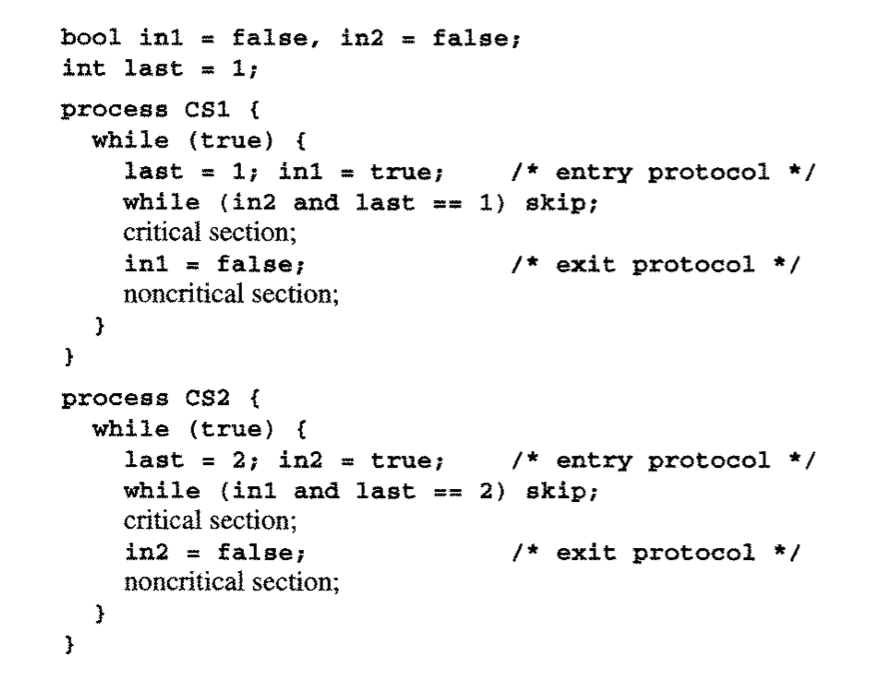
\includegraphics[scale=0.5]{tie-breaker.png}
    \caption{Algoritmo tie-breaker para dos procesos. (Andrews')}
  \end{figure}
\end{frame}

\begin{frame}
  \frametitle{Introducción: interleavings}
  \begin{itemize}
    \item En este terreno se sigue investigando para encontrar un modo definitivo que permita solucionar los problemas o detectarlos.
    \item Uno de los primeros asuntos estudiados es determinar el estado o estados finales a los que se llega ejecutando un programa concurrente.
  \end{itemize}
\end{frame}

\begin{frame}[fragile]
  \frametitle{Introducción: interleavings}
  \begin{lstlisting}
  int var;

  proc f1() {
    var := 1;
  }

  proc f2() {
    var := 2;
  }
  \end{lstlisting}
\end{frame}

\begin{frame}
  \frametitle{Introducción: interleavings}
  \begin{itemize}
  \item Explosión exponencial en el número de interleavings en proporción al número de hilos y al número de instrucciones.
  \item No siempre hay una correlación con el número de estados finales.
  \item No todos los interleavings tienen la misma importancia y algunos de ellos son equivalentes entre sí.
  \end{itemize}
\end{frame}

\begin{frame}[fragile]
  \frametitle{Introducción: interleavings}
  \begin{lstlisting}
  int var1;
  int var2;

  proc f1() {
    var1 := 1;  # 1
    var1 := 2;  # 2
  }

  proc f2() {
    var2 := 2;  # 3
    var2 := 1;  # 4
  }
  \end{lstlisting}
\end{frame}

\begin{frame}
  \frametitle{Introducción: grano}
  \begin{itemize}
  \item ¿Cuál es la atomicidad?
    \begin{itemize}
    \item Asignaciones atómicas: grano grueso.
    \item ¿Lectura de valores?: grano fino.
    \item ¡Secciones de código enteras!: \dots
    \end{itemize}
  \item ¿De qué depende el grano? ¿Qué ocurre si no hay memoria compartida?
  \end{itemize}
\end{frame}

\begin{frame}
  \frametitle{Introducción: actores}
  \begin{itemize}
  \item Cada objeto ejecuta sus tareas de forma concurrente con respecto a las del resto de objetos.
  \item Una única tarea a la vez por objeto. El resto de tareas esperan en una cola cuyo orden no es determinable.
  \item El paso de mensajes indica qué método desea ejecutar un objeto (pudiendo ser uno propio o perteneciente a otro objeto).
  \item Dependiendo del tipo de llamada, una tarea puede dejar paso a otra si aún no cuenta con los valores necesarios para proseguir.
  \item Se trata de una concurrencia donde el scheduler es non-preemptive.
  \end{itemize}
\end{frame}

\begin{frame}
  \frametitle{Introducción: ventajas}
  \begin{itemize}
  \item Reducción notable del número de interleavings: importante cuando se aplican técnicas de testing sistemático.
  \item Presente en lenguajes como Erlang, Scala y \textbf{ABS}.
  \item Cuenta con una amplia cantidad de herramientas, entre ellas, \textbf{SYCO}, que implementa \textbf{DPOR} para obtener los posibles resultados finales de un programa, reduciendo los interleavings redundantes.
  \end{itemize}
\end{frame}

\begin{frame}
  \frametitle{Introducción: objetivo}
  \begin{itemize}
  \item Acercar las herramientas de ABS a un lenguaje que no sea de modelado, como C.
  \item Un lenguaje que permita recrear una concurrencia entre procesos a nivel de grano fino.
  \item Un lenguaje sencillo pero completo: \textbf{CABS}.
  \end{itemize}
\end{frame}

\begin{frame}[fragile]
  \frametitle{CABS: sintaxis}
  \begin{itemize}
  \item Subconjunto de C con sintaxis para hebras.
  \item Tipos estáticos y arrays.
  \end{itemize}
  \lstinputlisting{code.0.1.txt}
\end{frame}

\begin{frame}[fragile]
  \frametitle{CABS: sintaxis}
  \begin{multicols}{2}
    \lstinputlisting{code.0.2.txt}
  \end{multicols}
\end{frame}

\begin{frame}[fragile]
  \frametitle{CABS: sintaxis}
  \lstinputlisting{code.0.3.txt}
\end{frame}

\begin{frame}
  \frametitle{CABS: semántica}
  \begin{itemize}
  \item Estado: $(\G, \F, \RP)$.
  \item Ámbito global de varibles ($\G$): asocia nombres de variables a valores de $\V$.
  \item Definición de funciones: $\F(\func) = (t, S_F, args_F, a_{ret})$.
  \item Lista de marcos de ejecución: $\RP \leadsto (local:s, S)$
  \end{itemize}
\end{frame}

\begin{frame}
  \frametitle{CABS: semántica}
  \fontsize{10}{7.2}\selectfont
  \begin{align*}
  \init(\varepsilon) &= (\nil, \nil, [])\\
  \init(int \var \; \P) &= (\G\ass{\var}{0}, \F, \RP) \\ &\text{ donde } \init(\P) = (\G, \F, \RP)\\
  \init(bool \var \; \P) &= (\G\ass{\var}{\False}, \F, \RP) \\ &\text{ donde } \init(\P) = (\G, \F, \RP)\\
  \init(int \, \func(\args) \{ S\; \return a\} \P) &= (\G, \F\ass{\func}{(int, S, \args, a)}, \RP) \\ &\text{ donde } \init(\P) = (\G, \F, \RP)\\
  \init(bool \, \func(\args) \{ S\; \return b\} \P) &= (\G, \F\ass{\func}{(bool, S, \args, b)}, \RP) \\ &\text{ donde } \init(\P) = (\G, \F, \RP)\\
  \init(void \, \func(\args) \{ S\} \P) &= (\G, \F\ass{\func}{(void, S, \args, \varepsilon)}, \RP) \\ &\text{ donde } \init(\P) = (\G, \F, \RP)\\
  \end{align*}
  $$
  \start((\G, \F, \RP)) = (\G, \F, [(\nil:[], S)]) \text{ donde } \F(main) = (int, S, \args, 0)
  $$
\end{frame}

\begin{frame}[fragile]
  \frametitle{CABS: semántica de las $\AExp$}
  \fontsize{10}{7.2}\selectfont
  \begin{prooftree*}
    \Infer[left label=$\numa$]0{\st{n}{(\G, \F, \RP \leadsto (s, S))} \staexp \st{\N \eval{n}}{(\G, \F, \RP \leadsto (s, S))}}
\end{prooftree*}

\begin{prooftree*}
        \hypo{local(x) = v}
    \Infer[left label=$\varal$]1{\st{x}{(\G, \F, \RP \leadsto (local:s, S))} \staexp \st{v}{(\G, \F, \RP \leadsto (local:s, S))}}
\end{prooftree*}

\begin{prooftree*}
        \hypo{G(x) = v}
        \hypo{local(x) = undef}
    \Infer[left label=$\varag$]2{\st{x}{(\G, \F, \RP \leadsto (local:s, S))} \staexp \st{v}{(\G, \F, \RP \leadsto (local:s, S))}}
\end{prooftree*}
\end{frame}

\begin{frame}[fragile]
  \frametitle{CABS: semántica de las $\AExp$}
  \fontsize{10}{7.2}\selectfont
\begin{prooftree*}
        \hypo{\st{a_1}{(\G, \F, \RP \leadsto (s, S))} \staexp \st{a_1'}{(\G, \F, \RP \leadsto (s', S'))}}
    \Infer[left label=$\opaa$]1{\st{a_1 \bigodot a_2}{(\G, \F, \RP \leadsto (s, S))} \staexp \st{a_1' \bigodot a_2}{(\G, \F, \RP \leadsto (s', S'))}}
\end{prooftree*}

\begin{prooftree*}
        \hypo{\st{a_2}{(\G, \F, \RP \leadsto (s, S)))} \staexp \st{a_2'}{(\G, \F, \RP \leadsto (s', S')))}}
    \Infer[left label=$\opab$]1{\st{v \bigodot a_2}{(\G, \F, \RP \leadsto (s, S)))} \staexp \st{v \bigodot a_2'}{(\G, \F, \RP \leadsto (s', S')))}}
\end{prooftree*}

\begin{prooftree*}
    \Infer[left label=$\opac$]0{\st{v_1 \bigodot v_2}{(\G, \F, \RP \leadsto (s, S))} \staexp \st{v_1 \bigodot_{\N} v_2}{(\G, \F, \RP \leadsto (s, S))}}
\end{prooftree*}
\end{frame}

\begin{frame}[fragile]
  \frametitle{CABS: semántica de las $\AExp$}
  \fontsize{7}{7.2}\selectfont
\begin{prooftree*}
        \hypo{\st{a}{(\G, \F, \RP \leadsto (s, S))} \staexp \st{a'}{(\G, \F, \RP \leadsto (s', S'))}}
    \Infer[left label=$\unaa$]1{\st{\Unstack{a}}{(\G, \F, \RP \leadsto (s, S))} \staexp \st{\Unstack{a'}}{(\G, \F, \RP \leadsto (s', S'))}}
\end{prooftree*}

\begin{prooftree*}
    \Infer[left label=$\unab$]0{\st{\Unstack{v}}{(\G, \F, \RP \leadsto (local:s, S))} \staexp \st{v}{(\G, \F, \RP \leadsto (s, S))}}
\end{prooftree*}

\begin{prooftree*}
      \hypo{\F(\func) = (int, S_F, args_F, a)}
      \hypo{check\_args(args_F, args)}
      \hypo{eval(args) = args'}
    \Infer[left label=$\callaa$]3{\st{\func(args)}{(\G, \F, \RP \leadsto (local:s, S))} \staexp \st{\func(args')}{(\G, \F, \RP \leadsto (local:s, S))}}
\end{prooftree*}

\fontsize{5}{7.2}\selectfont
\begin{prooftree*}
      \hypo{\F(\func) = (int, S_F, args_F, a)}
      \hypo{check\_args(args_F, args)}
      \hypo{eval(args) = v_1:\dots:v_n}
    \Infer[left label=$\callab$]3{\st{\func(args)}{(\G, \F, \RP \leadsto (local:s, S))} \staexp \st{\text{UNSTACK}(a)}{(\G, \F, \RP \leadsto (\nil\ass{args}{v_1:\dots:v_n}:local:s, S_F\;S))}}
\end{prooftree*}
\end{frame}

\begin{frame}[fragile]
  \frametitle{CABS: semántica de las asignaciones}
  \fontsize{8}{7.2}\selectfont
\begin{prooftree*}
        \hypo{\st{a}{(\G, \F, \RP \leadsto (local:s, \varepsilon))} \staexp \st{a'}{(\G, \F, \RP \leadsto (s', S_{\A}))}}
    \Infer[left label=$\assac$]1{(\G, \F, \RP \leadsto (local:s,\var = a\;S)) \stns (\G, \F, \RP \leadsto (s', S_{\A}\;\var = a'\;S))}
\end{prooftree*}

\begin{prooftree*}
        \hypo{is\_local(var)}
    \Infer[left label=$\assvc$]1{(\G, \F, \RP \leadsto (local:s,\var = v\;S)) \stns (\G, \F, \RP \leadsto (local\ass{\var}{v}:s, S))}
\end{prooftree*}

\begin{prooftree*}
        \hypo{is\_global(var)}
    \Infer[left label=$\assvcg$]1{(\G, \F, \RP \leadsto (local:s,\var = v\;S)) \stns (\G\ass{\var}{v}, \F, \RP \leadsto (local:s, S))}
\end{prooftree*}
\end{frame}

\begin{frame}[fragile]
  \frametitle{CABS: semántica del if}
  \fontsize{8}{7.2}\selectfont
\begin{prooftree*}
        \hypo{\st{b}{(\G, \F, \RP \leadsto (local:s, \varepsilon))} \stbexp \st{b'}{(\G, \F, \RP \leadsto (s', S_{\B}))}}
    \Infer[left label=$\ifac$]1{(\G, \F, \RP \leadsto (local:s, \If{b}{S_1}{S_2}S)) \stns (\G, \F, \RP \leadsto (s', S_{\B}\;\If{b'}{S_1}{S_2}S))}
\end{prooftree*}

\begin{prooftree*}
    \Infer[left label=$\iftc$]0{(\G, \F, \RP \leadsto (local:s, \If{\True}{S_1}{S_2}S)) \stns (\G, \F, \RP \leadsto (local:s, S_1\;S))}
\end{prooftree*}

\begin{prooftree*}
    \Infer[left label=$\iffc$]0{(\G, \F, \RP \leadsto (local:s, \If{\False}{S_1}{S_2}S)) \stns (\G, \F, \RP \leadsto (local:s, S_2\;S))}
\end{prooftree*}
\end{frame}

\begin{frame}[fragile]
  \frametitle{CABS: semántica del thread}
  \fontsize{8}{7.2}\selectfont
\begin{prooftree*}
    \Infer[left label=$\enac$]0{(\G, \F, \RP \leadsto (s, \varepsilon))) \stns (\G, \F, \RP))}
\end{prooftree*}

\begin{prooftree*}
      \hypo{\F(\func) = (t, S_F, args_F, e)}
      \hypo{check\_args(args_F, args)}
      \hypo{eval(args) = args'}
    \Infer[left label=$\threadca$]3{(\G, \F, \RP \leadsto (s, \thread \,\func(args)\;S)) \stns (\G, \F, (\RP \leadsto (s,  \thread \,\func(args')\;S))}
\end{prooftree*}

  \fontsize{6}{7.2}\selectfont
\begin{prooftree*}
      \hypo{\F(\func) = (t, S_F, args_F, e)}
      \hypo{check\_args(args_F, args)}
      \hypo{eval(args) = v_1:\dots:v_n}
    \Infer[left label=$\threadcb$]3{(\G, \F, \RP \leadsto (s, \thread \,\func(args)\;S)) \stns (\G, \F, (\RP \cup (\nil\ass{args}{v_1:\dots:v_n}:[], S_F)) \leadsto (s, S))}
\end{prooftree*}
\end{frame}

\begin{frame}[fragile]
  \frametitle{CABS: ejemplo}
  \lstinputlisting{code.0.3.txt}
\end{frame}

\begin{frame}[fragile]
  \frametitle{CABS: ejemplo}
  \fontsize{8}{7.2}\selectfont
  Excluyendo algunos pasos:
\begin{multline*}
  (\G, \F, (\nil, \thread \,f(1)\;\thread \,f(2)\;)) \stns \\
  (\G, \F, (\nil\ass{value}{1}, var = value\;):(\nil, \thread \,f(2)\;)) \stns \\
  (\G, \F, (\nil\ass{value}{1}, var = value\;):(\nil\ass{value}{2}, var = value\;):(\nil, \varepsilon)) \stns \\
  (\G\ass{var}{1}, \F, (\nil\ass{value}{1}, \varepsilon):(\nil\ass{value}{2}, var = value\;):(\nil, \varepsilon)) \stns \\
  (\G\ass{var}{2}, \F, (\nil\ass{value}{1}, \varepsilon):(\nil\ass{value}{2}, \varepsilon):(\nil, \varepsilon)) \stns \\
  (\G\ass{var}{2}, \F, [])
\end{multline*}
\end{frame}

\begin{frame}[fragile]
  \frametitle{ABS: sintaxis}
  \begin{itemize}
  \item Sintaxis parecida a la de Java (aproximadamente).
  \item Clases que implementan interfaces para exponer los métodos públicos.
  \item Tipos futuro para esperar resultados del paso de mensajes (await).
  \end{itemize}
  \fontsize{7}{7.2}\selectfont
  \lstinputlisting{code.1.1.txt}
  \lstinputlisting{code.1.2.txt}
  \lstinputlisting{code.1.3.txt}
\end{frame}

\begin{frame}[fragile]
  \frametitle{ABS: semántica}
 \begin{itemize}
  \item Estado: $(\O, \Cl)$.
  \item Definición de las clases: $\Cl\eval{c} = (\mbox{Inter}, attr_c, met, args_c)$.
  \item Lista de objetos instanciados (actores): $\O \leadsto (id, c, \RT \leadsto (loc, S, t), t, \attr)$
  \end{itemize}
\end{frame}

\begin{frame}[fragile]
  \frametitle{ABS: algunas reglas semánticas}
  \fontsize{5}{7.2}\selectfont
  \begin{prooftree*}
      \hypo {is\_local(x)}
      \hypo {is\_Int(x)}
    \Infer[left label=$\assa$]2{(\O \leadsto (id, c, \RT \leadsto (loc, x = a\; S, t), t, \attr), \Cl) \stns (\O \leadsto (id, c, \RT \leadsto (loc \ass{x}{\A \eval{a}_{loc, \attr}}, S, t), t, \attr), \Cl)}
  \end{prooftree*}

  \fontsize{4}{7.2}\selectfont
   \begin{prooftree*}
      \hypo{\Cl\eval{c'} = (\mbox{Inter}, attr_c, met, args_c)}
      \hypo{check\_args(args_c, args)}
    \Infer[left label=$\oabs$]2{(\O \leadsto (id, c, \RT \leadsto (loc,  \mbox{Inter } inter = new\, c'(args)\; S, t), t, \attr), \Cl) \stns (\O:o \leadsto (id, c, \RT \leadsto (loc \ass{inter}{id'}, S, t), t, \attr), \Cl)}
   \end{prooftree*}
\fontsize{7}{7.2}\selectfont
   donde $o = (id', c', [], \perp, \attr')$ con $id'$ un nuevo identificador de objeto no utilizado y $\attr' = attr_c \ass{args_c}{\E\eval{args}_{loc, \attr}}$ los atributos del nuevo objeto creado.
\end{frame}

\begin{frame}[fragile]
  \frametitle{ABS: algunas reglas semánticas}
  \fontsize{5}{7.2}\selectfont
\begin{prooftree*}
      \hypo{loc \cup attr \eval{int} = id'}
      \hypo{\Cl\eval{c'} = (\mbox{Inter}, attr_c, met, args_c)}
      \hypo{contains(met, m)}
      \hypo{check\_args(args_m, args)}
    \Infer[left label=$\tskabsb$]4{(\O \leadsto  (id', c', \RT', t', \attr') (id, c, \RT \leadsto (loc, Int\,x = await\,int!m(args)\; S, t), t, \attr), \Cl) \stns st}
\end{prooftree*}
 \fontsize{7}{7.2}\selectfont
 donde $o' = (id', c', \RT':tsk, t', \attr')$, $tsk = (loc', S', t'')$ con $t''$ un identificador de tarea nuevo y $loc' = \nil\ass{args_m}{args}$, $met\eval{m} = (S', args_m)$ y $st = (\O \leadsto o' (id, c, \RT \leadsto (loc, Int\,x = await\,t'\; S, t), t, \attr), \Cl)$

 \begin{prooftree*}
      \hypo{tsk = (loc', \varepsilon(\nu), t'')}
    \Infer[left label=$\retabs$]1{(\O \leadsto  (id', c', \RT' \leadsto tsk, t', \attr') (id, c, \RT \leadsto (loc, Int\,x = await\,t'\; S, t), t, \attr), \Cl) \stns st}
  \end{prooftree*} donde $o' = (id', c', \RT', t', \attr')$ y $st = (\O \leadsto o' (id, c, \RT \leadsto (loc\ass{x}{\nu}, S, t), t, \attr), \Cl)$

 \fontsize{6}{7.2}\selectfont
 \begin{prooftree*}
    \Infer[left label=$\eabs$]0{(\O \leadsto (id, c, \RT \leadsto (loc, \return a\;S, t), t, \attr), \Cl) \stns (\O \leadsto (id, c, \RT \leadsto (loc, \varepsilon(\A \eval{a}_{loc, \attr}), t), \perp, \attr), \Cl)}
  \end{prooftree*}
\end{frame}

\begin{frame}[fragile]
  \frametitle{ABS: ejemplo}
  \fontsize{5}{7.2}\selectfont
   \begin{multicols}{2}
     \lstinputlisting{code.1.6.txt}
   \end{multicols}
\end{frame}

\begin{frame}[fragile]
  \frametitle{Traducción}
  \begin{itemize}
  \item Necesitamos crear de forma artificial un ámbito global de variables (memoria compartida ausente en ABS).
  \item La traducción de las funciones y procedimientos tienen que ser visibles desde cualquier punto del programa (¿métodos públicos de interfaz o métodos privados de una única clase?).
  \item La concurrencia tiene que ser de grano fino (ABS implementa el modelo de actores).
  \item Hay que dar un soporte a los arrays en ámbito local y global (ABS tiene un tipo de lista enlazada).
  \end{itemize}
\end{frame}

\begin{frame}[fragile]
  \frametitle{Traducción: ámbito global de variables y funciones}
  \fontsize{5}{7.2}\selectfont
  \begin{multicols}{2}
    \lstinputlisting{example.txt}
    \vfill
    \fontsize{10}{7.2}\selectfont
    Así solo es posible un interleaving.\\
    \vfill
    Tal vez usando:
    \fontsize{5}{7.2}\selectfont
    \begin{lstlisting}
    this!f();
    suspend;
    \end{lstlisting}
    \vfill\null
    \columnbreak
    \lstinputlisting{code.2.1.txt}
  \end{multicols}
\end{frame}

\begin{frame}[fragile]
  \frametitle{Traducción: ámbito global de variables y funciones}
  Tampoco funciona la idea del \emph{suspend}
  {\fontsize{6}{7.2}\selectfont
    \lstinputlisting{code.2.2.txt}}
  Concluimos que cada función tiene que ir en un objeto distinto.
\end{frame}

\begin{frame}[fragile]
  \frametitle{Traducción: ámbito global de variables y funciones}
  ¿Qué hacemos ahora con las variables globales? Ya no pueden ser atributos de una clase que implemente una función. Necesita su propio objeto.
  \begin{multicols}{2}
  {\fontsize{6}{7.2}\selectfont
    \lstinputlisting[firstline=1,lastline=30]{code.2.3.txt}}
  \end{multicols}
  Usaremos llamadas asíncronas para manejar este objeto:
  \fontsize{6}{7.2}\selectfont
  \begin{lstlisting}
  globalval!setvar(1);
  Int x = await globalval!getvar();
  \end{lstlisting}
\end{frame}

\begin{frame}[fragile]
  \frametitle{Traducción: arrays locales y globales}
  El mismo argumento que hemos empleado para las variables globales (preservación de los interleavings) se puede aplicar a los arrays encapsulando una lista de ABS en una clase.
  \begin{multicols}{2}
  {\fontsize{6}{7.2}\selectfont
    \lstinputlisting{code.2.4.txt}}
  \end{multicols}
  Para el ámbito global hay que añadir algunos métodos extra (\emph{retrievearray}, \emph{init} \dots).
\end{frame}

\begin{frame}[fragile]
  \frametitle{Traducción: función de traducción $\AExp$}
  \begin{figure}[h]
    \centering
    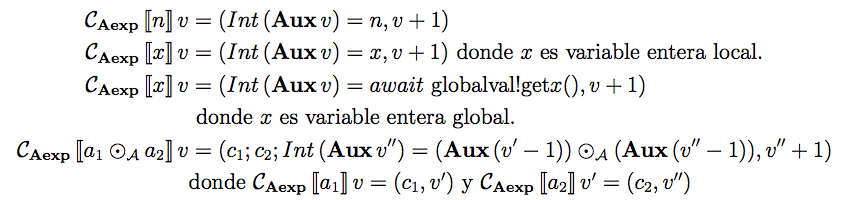
\includegraphics[scale=0.7]{trada.png}
  \end{figure}
  \begin{figure}[h]
    \centering
    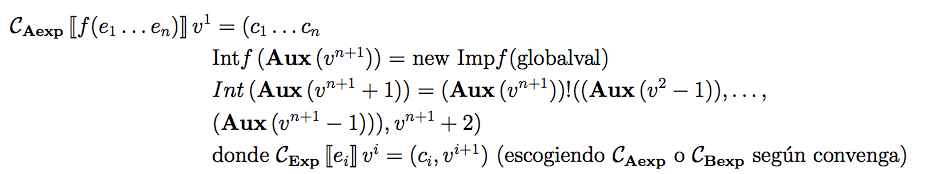
\includegraphics[scale=0.7]{tradf.png}
  \end{figure}
\end{frame}

\begin{frame}[fragile]
  \frametitle{Traducción: función de traducción del if y del while}
  \begin{figure}[h]
    \centering
    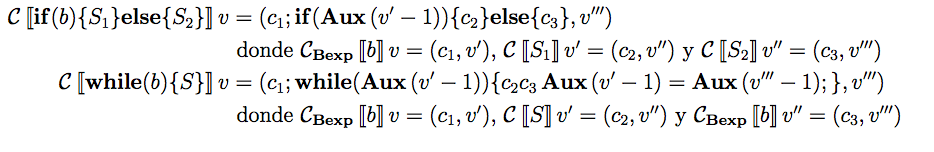
\includegraphics[scale=0.7]{tradc.png}
  \end{figure}
\end{frame}

\begin{frame}[fragile]
  \frametitle{Traducción: función de traducción de una función y del thread}
  \begin{figure}[h]
    \centering
    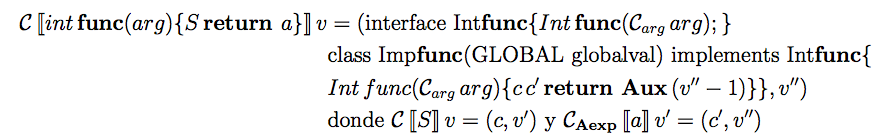
\includegraphics[scale=0.7]{tradfd.png}
  \end{figure}
  \begin{figure}[h]
    \centering
    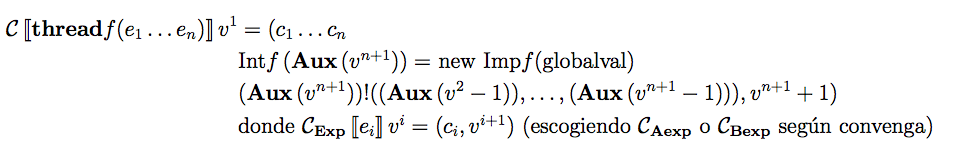
\includegraphics[scale=0.7]{tradth.png}
  \end{figure}
\end{frame}

\end{document}
